\documentclass{article}
\usepackage{listings}
\usepackage[usenames,dvipsnames]{color}
\usepackage{amsmath}
\usepackage[parfill]{parskip}
\usepackage{graphicx}
\usepackage{bm}
\usepackage{ifthen}
\usepackage{cite}
\usepackage{float}
\lstset{
  language=python,                     % the language of the code
  basicstyle=\ttfamily, % the size of the fonts that are used for the code
}
\newcommand\norm[1]{\left\lVert#1\right\rVert}
\usepackage{hyperref}
\hypersetup{
    colorlinks=true,
    urlcolor=blue,
    citecolor=black,
    linkcolor=black
}
\usepackage[a4paper]{geometry}
\begin{document}

\title{Gaussian processes and Gauss Markov random fields}
\date{\today}
\author{Tudor Muntianu}
\maketitle

\begin{abstract}
This report gives a (very) brief summary of work done this term while taking David
Blei's course, Foundations of Graphical Models, as administered and supervised
by Jeremy. The \href{https://github.com/tmuntianu/gmrfs}{GitHub repo} contains
all of the code and notebooks that I'll reference here. Some of them are quite
messy because they are still being tinkered with.
\end{abstract}

\section{Motivation}
The primary motivation for this independent study was the SuperEEG project, which
is based largely on Gaussian process regression. Currently the model does not
rely on much of the state-of-the-art for GPs largely due to the structure of
the problem and the resulting difficulty in expressing it as a single covariance
matrix. So the work from this term can be seen as an attempt to take a second
crack at this problem while also gaining a (more) solid foundation in graphical
models.

So rather than examine any dataset or problem (even ECoG data specifically)
in particular, I wanted to explore and learn more about graphical models, GMRfs, GPs, VI, and the
software packages that implement them, largely because a SuperEEG 2.0 would
call for using something other than NumPy for computation.

\section{The problem}
The basic idea of SuperEEG is to impute spatial data at locally unobserved
but globally observed locations, and using this global structure to improve these
imputed values. There are not enough papers on this subject, and many of them
come from the field of geostatistics where locations are never observed globally.
In ECoG at some point every location in sampled, but that is not the case on Earth.
This is why GPs can be used in geostatistics, see Alvarez's review\cite{alvarez2012kernels} which contains some examples,
and why SuperEEG's flavor of GPs is novel.

There are, however, some developments which have bled over from computer vision.
Deep GMRFs\cite{deepgmrf} and other inpainting models (which are really just
imputing values in images like deep image priors\cite{dip} offer some interesting
perspectives on this sort of spatial imputation.
So what I did here was 1) implement a relatively simple but very powerful GP
architecture to learn some variational inference and some other GP-specific
methods such as inducing point methods, and 2) reimplement the Siden and Lindsten's deep GMRF model
because their code is... neither particularly extensible nor readable. I also picked
this model because there are a number of clear future directions that are not as
difficult as in the world of theoretical GPs (which is astonishingly deep
and convoluted).

\section{Image classification and GPs}
For the GP part of the term, I chose to implement and play with van der Wilk's
convolutional Gaussian processe.
van der Wilk's paper is significant because of the historical Gaussian process
struggle with images. This struggle originates from two facts: 1) GPs are $\mathcal{O}
(n^3)$ for training, and require $\mathcal{O}(n^2)$ memory, making dealing with
thousands of images times thousands of pixels difficult, and 2) many
traditional/commonly used kernels are stationary (translation invariant), making it difficult
for them to capture image structure in the way CNNs and other deep architectures
can. These limitations are not unique to images, but with MNIST and CIFAR being
common datasets, the limitations of GPs are quickly seen when applied to these.
However, variational inference and sparse approximations have done much to alleviate the first issue, and newer
state-of-the-art methods like deep kernel learning \cite{wilson} and deep convolutional
GPs \cite{deepconv} have been tackling the second.

The way shallow convolutional GPs attack this problem is in much the same way. The
model uses inducing points and stochastic VI to make training and inference possible,
and the structure of the convolutional kernel allows the stationary radial basis
function to also acquire certain non-stationary properties by operating on individual
patches and taking weighted sums over them. The exact mechanism of this operation
will be described later, but intuitively, it allows the kernel to express relationships
between distant pixels while also encoding information about proximal pixels
through the RBF. It's a useful (albeit at this point dated) extension of CNNs to GPs
much in the same way Siden's deep GMRF paper does the same thing for GMRFs.

\section{Deep GMRFs and inpainting}
A brief introduction to GMRFs is simple: a GMRF is just a random vector from
a multivariate Gaussian that satisfies certain conditional independence assumptions.
These assumptions can be modified depending on the context, but are always present
(hence Gauss Markov). See Rue and Held for more\cite{gmrf}. These models have been largely ignored as they relied largely
on the advantage that the representing precision matrices are sparse, and so
clever numerical algorithms to operate efficiently on these matrices yielded
good results in the past. Obviously this advantage diminishes daily now that
we have great autodiff and better/easier sampling tools.

Nevertheless GMRFs are probabalistic graphical models that can carry forward
uncertainty estimates, while also benefiting from VI techniques, so they still
have utility albeit not in their most rudimentary forms.

The deep GMRF model is simple, though interestingly it defines the generative
process ``backwards''. The process is as follows (ignoring
many details of the CNN), given
an image with missing pixels:
\begin{enumerate}
	\item Sample from a GMRF with the image as a mean, and $\sigma^2 \bm{I}$
	as the covariance, where $\sigma^2$ is a learned parameter
	\item Put this sample through a (special) CNN such that the output is
	a GMRF distributed according to $\mathcal{N}(\bm{0},\bm{I})$
\end{enumerate}
Intuitively then this process if just sampling a standard normal GMRF and then
sending it backwards through a CNN to get the image, though in this case the latent
variables we are learning are the pixels of the image regardless of whether they
are missing.

\section{Quick summary of current state of notebooks}
The GP notebooks are readable and pretty self-explanatory, so I'm not going to
discuss them much here. I also think the GMRF direction is more interesting
anyway.

There is a \lstinline{convgps} folder in the GP notebook
folder that contains the GPyTorch implementation of convolutional kernels.

The notebooks are a bit of a mess since I'm still breaking everything.
Here are the results so far.

\begin{figure}[H]
	\begin{tabular}{c c c}
		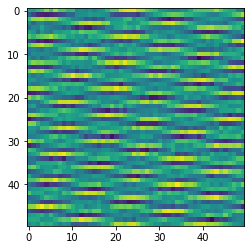
\includegraphics[width=0.33\linewidth]{images/original.png} &
		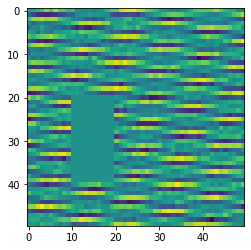
\includegraphics[width=0.33\linewidth]{images/masked.png} &
		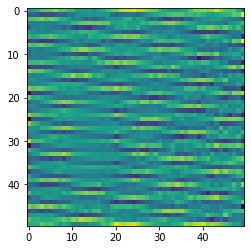
\includegraphics[width=0.33\linewidth]{images/inpainted.png}
	\end{tabular}
	\caption{From left to right: original image, masked image, posterior VI mean}
\end{figure}

The results of the VI mean are surprisingly good, especially given what the
Siden paper reports. They use a diagonal multivariate Gaussian as the variational
distribution, and admit that this is a very restrictive distribution.
Their reasoning is that they use VI only to learn the model parameters, and then
they use conjugate gradient to actually sample the posterior. This works because
the CNN constraints they describe requires that the transformation be full rank
in order to produce a valid GMRF. Then you can just pretend that the entire
CNN is one matrix and perform CG to get a solution, which gives a way of getting
the posterior mean and variance, as well as allowing sampling.

I've included my own CG implementation in the notebook but have not adapted it
to the CNN mostly because this method is extremely inelegant. Using VI just to optimize
model parameters and then using a linear system solver (on what is ultimately
a non-linear transform if using ReLU or any non-linear activation function) to
sample the posterior is redundant. The authors admit this, but still rather than
replicate the same hack they did I'd rather try to improve the variational distribution.

Regardless, the image above is just a bunch of sine and cosine functions (see
notebooks for details), and part of the image is masked. Using the same diagonal
multivariate Gaussian variational distribution, though, the model still managed
to achieve impressive inpainting, although it added significant noise to the image.
Rather than play around with more parameters to reduce this noise, though, I'm
currently trying to come up with a more expressive variational distribution, especially
since Pyro allows very flexible creations of variational distribution or ``guides.''

Another really interesting observation is that the missing pixels are learned
earlier than than the observed pixels.
\begin{figure}[H]
	\begin{center}
		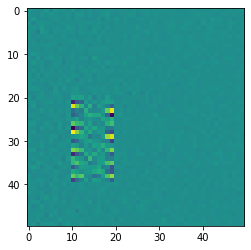
\includegraphics[width=0.5\linewidth]{images/iter1000.png}
	\end{center}
	\caption{Variational posterior mean at iteration 1000 of training}
\end{figure}
This indicates again that the variational distribution is the limiting factor,
since it constrains the existing pixels rather than the missing ones, while the model
itself
is able to quickly learn the structure and begin imputing well even after limited
training.

Apart from coming up with a better variational distribution, there's some more
changes that might be made. The current model only operates on one image, though
since the CNN parameters hopefully learn the global structure, we could treat
each image as conditionally independent and then optimize these parameters (or
a superset of them created to better deal with multiple images) in order to
train on different sets of imputed pixels.

So these are the two areas for more work: 1) better variational distribution,
2) extend the model to allow conditional independence of images with different
masks or missing pixels.

\section{Quick note on GPyTorch and GPFlow}
When implementing the conv GPs, I looked at van der Wilk's implementations in
GPFlow, a TensorFlow based GP library. I intentionally chose GPyTorch to make
it harder for myself (no cheating or copy-paste), but also so that I could compare the two.

While I prefer GPFlow due to the sheer readablity of the
existing code, and the large array of models already implemented, I think GPyTorch
has a more powerful stack. Integration with Pyro makes MCMC and VI stupid easy (and Stan borderline irrelevant), more sophisticated lazy and approximate covariance calculations are powerful but difficult to leverage for custom models, although the developers respond to requests for help or features quickly.
GPyTorch is also seeing significant development activity and funding, so I would expect
it to continue to outpace GPFlow from a technical perspective, but perhaps not from
a usability perspective.

Both are crucially missing basic explanations of how and where inference lives in
the model, kernel, and likelihood objects. This makes building truly custom models from scratch
extremely painful the first time around. I spent at least five hours just reading
through the codebases in an attempt to decipher the package's architecture.
Pyro is much the same way. Once you need to implement a custom loss function or
change the way the ELBO is computed docs get thin and examples are not found.

\nocite{*}
\bibliography{bib}
\bibliographystyle{plain}

\end{document}
